\input templates/header
\title[ASD - Backtracking]{\textbf{Algoritmi e Strutture Dati}\\[24pt]Backtracking}

\usepackage[mode=buildnew]{standalone}
\usepackage{xcolor}
\usepackage{colortbl}
\usepackage{epigraph}
\usepackage{tikz}
\usepackage{xmpmulti}
\usepackage{listings}

\lstset{
  basicstyle=\ttfamily,
  columns=fullflexible,
  keywordstyle=\color{red}\bfseries,
  commentstyle=\color{blue},
  showstringspaces=false,
}

\newcommand{\R}[1]{\textcolor{red}{#1}}
\newcommand{\B}[1]{\textcolor{blue}{#1}}

\renewcommand{\arraystretch}{1.4}
\graphicspath{{figs/16/}}

\renewcommand{\enumerazione}{\fontproc{enumeration}}
\newcommand{\isAdmissible}{\fontproc{isAdmissible}}

\begin{document}


%-------------------------------------------------------------------------
\FrameTitle{}

%-------------------------------------------------------------------------
\FrameContent



%%%%%%%%%%%%%%%%%%%%%%%%%%%%%%%%%%%%%%%%%%%%%%%%%%%%%%%%%%%%%%%%%%%%%%%%%%
\section{Introduzione}

%-------------------------------------------------------------------------
\begin{frame}{Introduzione}

\vspace{-9pt}
\BB{Classi di problemi (decisionali, di ricerca, di ottimizzazione)}

\BI
\item Definizioni basate sul concetto di \alert{soluzione ammissibile}: una soluzione
che soddisfa un certo insieme di criteri
\EI

\BB{Problemi tipici}
\BI
\item Costruire almeno una o tutte le soluzioni ammissibili
\item Contare le soluzioni ammissibili
\item Trovare le soluzioni ammissibili "più grandi", "più piccole" o in generale "ottimali"
\EI

\end{frame}


%-------------------------------------------------------------------------
\begin{frame}{Problemi tipici}

\vspace{-9pt}
\begin{myboxtitle}[Enumerazione]
\BIL
\item Elencare algoritmicamente tutte le soluzioni ammissibili (spazio di ricerca)
\item Esempio: elencare tutte le permutazioni di un insieme
\EIL
\end{myboxtitle}

\begin{myboxtitle}[Costruire almeno una soluzione]
\BIL
\item Si utilizza l'algoritmo per l'enumerazione, fermandosi alla prima soluzione 
disponibile
\item Esempio: identificare una sequenza di mosse nel gioco del 15
\EIL
\end{myboxtitle}

\end{frame}

%-------------------------------------------------------------------------
\begin{frame}{Problemi tipici}

\vspace{-9pt}
\begin{myboxtitle}[Contare le soluzioni]

\medskip
\TwoCols{
\BIL
\item In alcuni casi, è possibile contare in modo analitico
\item Esempio: contare il numero di sottoinsiemi di $k$ elementi presi da un 
insieme di $n$ elementi
\[
  \frac{n!}{k!\,(n-k)!}
\]
\EIL
}{
\BIL
\item In altri casi, si costruiscono le soluzioni e si contano
\item Esempio: numero di sottoinsiemi di un insieme di interi $S$ la cui somma
è un numero primo.
\EI
}
\end{myboxtitle}

\end{frame}


%-------------------------------------------------------------------------
\begin{frame}{Problemi tipici}

\vspace{-9pt}
\begin{myboxtitle}[Trovare le soluzioni ottimali]
\BIL
\item Si enumerano tutte le soluzioni, che vengono valutate tramite una
funzione di costo
\item Si possono utilizzare altre tecniche:
	\BI
	\item Prog. dinamica, greedy
	\item Tecniche risolutive per problemi intrattabili
	\EI
\item Esempio: Circuito hamiltoniano (commesso viaggiatore)
\EIL
\end{myboxtitle}


\end{frame}

\begin{frame}{Costruire tutte le soluzioni}

\vspace{-9pt}
\begin{myboxtitle}[Brute-force]
Un approccio per costruire tutte le soluzioni
\end{myboxtitle}



\BIL
\item Si esamina interamente lo spazio delle possibili soluzioni
\item A volte è l'unica strada possibile
\item La potenza dei computer moderni rende "affrontabili" problemi di dimensioni medio-piccole
\BI
\item $10!	= 3.63 \cdot 10^6$	(permutazione di 10 elementi)
\item $2^{20} = 1.05 \cdot 10^6$ (sottoinsieme di 20 elementi)
\EI
\item  Inoltre, a volte lo spazio delle soluzioni non deve essere analizzato 
interamente
\EIL
\end{frame}

%-------------------------------------------------------------------------
\begin{frame}{Backtracking}

\vspace{-9pt}
\begin{myboxtitle}[Filosofia]
\BIL
\item  "\emph{Prova a fare qualcosa, e se non va bene, disfalo e prova qualcos'altro}"
\item "\emph{Ritenta, e sarai più fortunato}"
\EIL
\end{myboxtitle}

\begin{myboxtitle}[Come funziona?]
\BI
\item Un metodo sistematico per iterare su tutte le possibili istanze di uno spazio di ricerca
\item E' una tecnica algoritmica che, come altre, deve essere personalizzata per ogni applicazione individuale
\EI
\end{myboxtitle}

\end{frame}


\begin{frame}{Organizzazione generale}
    
\begin{myboxtitle}[Organizzazione generale]
\BI
\item Una soluzione viene rappresentata come un \alert{vettore $S[1 \ldots n]$} 
\item  Il contenuto degli elementi $S[i]$ è preso da un \alert{insieme di scelte $C$} dipendente dal problema
\EI
\end{myboxtitle}

\begin{myboxtitle}[Esempi]
\BI
\item $C$ insieme generico, possibili soluzioni \alert{permutazioni} di $C$
\item $C$ insieme generico, possibili soluzioni \alert{sottoinsiemi} di $C$
\item $C$ mosse di gioco, possibili soluzioni \alert{sequenze di mosse}
\item $C$ archi di un grafo, possibili soluzioni \alert{percorsi sul grafo}
\EI
\end{myboxtitle}

\end{frame}

\begin{frame}{Soluzioni parziali}

\BIL
\item Ad ogni passo, partiamo da una soluzione parziale $S[1 \ldots k]$ in cui
$k \geq 0$ scelte sono state prese
\item Se $S[1 \ldots k]$ è una soluzione ammissibile, la "processiamo" 
  \BI
	\item Viene stampata, contata, evaluata
	\item Si può decidere di terminare o continuare elencando tutte le soluzioni
	\EI
\item Se $S[1 \ldots k]$ non è una soluzione completa
  \BI
  \item Se è possibile, estendiamo $S[1 \ldots k]$ con una delle possibili 
	  scelte in una soluzione $S[1 \ldots k+1]$
	\item Altrimenti, "cancelliamo" l'elemento $S[k]$ (backtrack) 
	e ripartiamo dalla soluzione $S[1 \ldots k-1]$
  \EI
\EIL

\end{frame}

\begin{frame}{Albero delle decisioni}

\BI
\item \alert{Albero di decisione} $\equiv$ Spazio di ricerca
\item \alert{Radice} $\equiv$ Soluzione parziale vuota
\item \alert{Nodi interni dell'albero di decisione} $\equiv$ Soluzioni parziali  
\item \alert{Foglie in un albero di decisione} $\equiv$ Soluzioni ammissibili 
\EI

\medskip
\begin{overprint}
\onslide<1|handout:0>\centerline{\includestandalone{figs/16/albero01}}
\onslide<2|handout:0>\centerline{\includestandalone{figs/16/albero02}}
\onslide<3|handout:0>\centerline{\includestandalone{figs/16/albero03}}
\onslide<4|handout:0>\centerline{\includestandalone{figs/16/albero04}}
\onslide<5|handout:0>\centerline{\includestandalone{figs/16/albero05}}
\onslide<6|handout:0>\centerline{\includestandalone{figs/16/albero06}}
\onslide<7|handout:0>\centerline{\includestandalone{figs/16/albero07}}
\onslide<8|handout:0>\centerline{\includestandalone{figs/16/albero08}}
\onslide<9|handout:0>\centerline{\includestandalone{figs/16/albero09}}
\onslide<10|handout:1>\centerline{\includestandalone{figs/16/albero10}}
\end{overprint}

\end{frame}

\begin{frame}{Pruning}

\BI
\item “Rami” dell'albero che sicuramente non portano a soluzioni ammissibili possono essere “\alert{potati}”  (\alert{pruned})
\item La valutazione viene fatta nelle soluzioni parziali radici del sottoalbero da potare
\EI

\begin{overprint}
\onslide<1|handout:0>\centerline{\includestandalone{figs/16/pruning1}}
\onslide<2|handout:1>\centerline{\includestandalone{figs/16/pruning2}}
\end{overprint}

\end{frame}

\begin{frame}{Backtracking - Due possibili approcci}

\vspace{-9pt}
\begin{myboxtitle}[Ricorsivo]
\BIL
\item Lavora tramite una visita in profondità nell'albero delle scelte, basata su un approccio ricorsivo
\EIL
\end{myboxtitle}


\begin{myboxtitle}[Iterativo]
\BIL
\item Utilizza un approccio greedy, eventualmente tornando sui propri passi
\item Esempio: \alert{Inviluppo convesso}
\item Esempio: \alert{String matching}
\EIL
\end{myboxtitle}

\end{frame}

\section{Enumerazione}


\begin{frame}{Enumerazione}

\vspace{-9pt}
\begin{Procedure}
\caption[A]{\BOOLEAN\ \enumerazione($\Item[\,]\ S$, \INTEGER $n$, \INTEGER\ $i$, \mldots)}
\Comment{Determina $C$ in funzione di $S[1 \mldots i-1]$}
$\Set\ C = \getChoices(S, n, i, \mldots)$\;
\ForEach{$c \in C$}
{
  $S[i] = c$\;
  \If{$\isAdmissible(S, n, i)$}
  {
    \If{$\processSolution(S, n, i, \mldots)$}{\Return \TRUE}
  }
  \If{$\enumerazione(S, n, i+1, \mldots)$}{\Return\ \TRUE}
}
\Return \FALSE\;
\end{Procedure}

\end{frame}

\begin{frame}{Enumerazione}

\BIL
\item $S$: vettore contenente le soluzioni parziali $S[1 \ldots i]$
\item $i$: indice corrente
\item $\mldots$: informazioni addizionali
\item $C$ è l'insieme dei possibili candidati per estendere la soluzione
\item $\isAdmissible()$: restituisce \TRUE se $S[1 \ldots i]$ è una soluzione ammissibile
\item $\processSolution()$: restituisce 
\BI
\item \TRUE per bloccare l'esecuzione alla prima 
soluzione ammissibile, 
\item \FALSE per esplorare tutto l'albero
\EI
\EIL

\end{frame}

\subsection{Sottoinsiemi}

\begin{frame}{Esempio 1}

\BB{Elencare tutti i sottoinsiemi dell'insieme $\{ 1, \ldots, n \}$}

\begin{Procedure}
\caption[A]{\enumerasottoinsiemi($\INTEGER[\,]\ S$, \INTEGER $n$, \INTEGER $i$)}
$\Set\ C = \IIF(i \leq n, \{ 0, 1 \}, \emptyset)$\;
\ForEach{$c \in C$}
{
  $S[i] = c$\;
  \If{$i \Eq n$}
  {
    $\processSolution(S,n)$\;
  }
  $\enumerasottoinsiemi(S, n, i+1)$\;
}
\end{Procedure}


\end{frame}

\begin{frame}{Esempio 1 (Versione più "pulita")}

\BB{Elencare tutti i sottoinsiemi dell'insieme $\{ 1, \ldots, n \}$}

\begin{Procedure}
\caption[A]{\enumerasottoinsiemi($\INTEGER[\,]\ S$, \INTEGER $n$, \INTEGER $i$)}
\eIf{$i \Eq n+1$}{
  $\processSolution(S,n)$\;
}{
  \ForEach{$c \in \{ 0, 1 \}$}{
    $S[i] = c$\;
  	$\enumerasottoinsiemi(S, n, i+1)$\;
  }
}
\end{Procedure}

\end{frame}

\begin{frame}{Esempio 1}
	
\BIL
\item Non c'è pruning. Tutto lo spazio possibile viene esplorato.\\
Ma questo avviene per definizione
\item Complessità $O(n 2^n)$
\item In che ordine vengono stampati gli insiemi?
\item E' possibile pensare ad una soluzione iterativa, ad-hoc?\\
(non-backtracking)
\EIL

\end{frame}

\begin{frame}{Esempio 1}

\begin{Procedure}
\caption[A]{\enumerasottoinsiemi(\INTEGER $n$)}
\For{$j = 0$ \TO $2^{n}-1$}{
  \PRINT\ '\{'\;
  \For{$i = 0$ \TO $n-1$}{
    \If{($j$ \AND $2^i) \neq 0$}{
      \PRINT\ $i$\;
    }
  }
  \PRINT\ '\}'\;
}
\end{Procedure}


\end{frame}


\begin{frame}{Esempio 2}

\BB{Elencare tutti i sottoinsiemi di $k$ elementi di un insieme $\{ 1, \ldots, n \}$}

\BIL
\item Versione iterativa
\BI
\item Qual è il costo?
\EI
\item Soluzione basata su backtracking
\BI
\item Possiamo potare?
\EI
\EIL


\end{frame}

\begin{frame}{Esempio 2 - Tentativo 1}

\begin{Procedure}
\caption[A]{\enumerasottoinsiemi($\INTEGER[\,]\ S$, \INTEGER $n$, \INTEGER $k$, \INTEGER $i$)}
$\Set\ C = \IIF(i \leq n, \{ 0, 1 \}, \emptyset)$\;
\ForEach{$c \in C$}
{
  $S[i] = c$\;
  \If{$i \Eq n$}
  {
    $\INTEGER\ \Count = 0$\;
    \For{$j = 1$ \TO $n$}{
       $\Count = \Count + S[j]$\;
    }
    \If{$\Count \Eq k$}{
      $\processSolution(S, n)$\;
    }
  }
  $\enumerasottoinsiemi(S, n, k, i+1)$\;
}
\end{Procedure}

\end{frame}

\begin{frame}{Esempio 2 - Tentativo 2}
	
\begin{Procedure}
\caption[A]{\enumerasottoinsiemi($\INTEGER[\,]\ S$, \INTEGER $n$, \INTEGER $k$, \INTEGER $i$, \INTEGER \Count)}
$\Set\ C = \IIF(i \leq n, \{ 0, 1 \}, \emptyset)$\;
\ForEach{$c \in C$}
{
  $S[i] = c$\;
  $\Count = \Count + S[i]$\;
  \If{$i \Eq n$ \AND\ $\Count \Eq k$}
  {
    $\processSolution(S,n)$\;
  }
  $\enumerasottoinsiemi(S, n, k, i+1, \Count)$\;
  $\Count = \Count - S[i]$\;
}
\end{Procedure}


\end{frame}

\begin{frame}{Esempio 2 - Tentativo 3 (Corretto)}

\begin{Procedure}
\caption[A]{\enumerasottoinsiemi($\INTEGER[\,]\ S$, \INTEGER $n$, \INTEGER $k$, \INTEGER $i$, \INTEGER \Count)}
$\Set\ C = \IIF(\Count < k$ \AND\ $\Count + (n-i+1) \geq k, \{ 0, 1 \}, \emptyset)$\;
\ForEach{$c \in C$}
{
  $S[i] = c$\;
  $\Count = \Count + S[i]$\;
  \eIf{$\Count = k$}
  {
    $\processSolution(S,i)$\;
  }{
    $\enumerasottoinsiemi(S, n, k, i+1, \Count)$\;
  }
  $\Count = \Count - S[i]$\;
}
\end{Procedure}

\end{frame}

\begin{frame}{Esempio 2: vantaggi}

\IG{1.0}{plot.pdf}

\end{frame}

\begin{frame}{Esempio 2 - Sommario}

\BB{Cosa abbiamo imparato?}
\BIL
\item  “Specializzando” l'algoritmo generico, possiamo ottenere una versione più efficiente
\item  Versione efficiente per 
\BI
	\item valori di $k$ “piccoli” (vicini a $1$)
	\item valori di $k$ “grandi” (vicini a $n$)
\EI
\item Miglioramento solo parziale verso $n/2$
\item E' difficile ottenere la stessa efficienza con un algoritmo iterativo
\EIL
	
\end{frame}

\subsection{Permutazioni}

\begin{frame}{Esempio 3}

\BB{Stampa di tutte le permutazioni di un insieme $A$}
\BI
\item L'insieme dei candidati dipende dalla soluzione parziale corrente
\EI

\begin{Procedure}
\caption[A]{\permutazioni(\Set $A$, \INTEGER $n$, $\Item[\,]\ S$, \INTEGER\ $i$)}
\ForEach{$c \in A$}{
  $S[i] = c$\;
  $A.\setremove(c)$\;
  \eIf{$A.\setempty()$}{
    $\processSolution(S, n)$
  }{
  	$\permutazioni(A, n, S, i+1)$\;
	}
  $A.\setinsert(c)$\;
}
\end{Procedure}

	
	
	
\end{frame}


\subsection{Giochi}

%-------------------------------------------------------------------------
\begin{frame}{Problema delle otto regine}

\vspace{-9pt}
\begin{myboxtitle}[Problema]
Posizionare $n$ regine in una scacchiera $n \times n$, in modo tale che 
nessuna regina ne "minacci" un'altra. 
\end{myboxtitle}

\TwoCols{
\BIL
\item Un po' di storia:
\BI
\item Introdotto da Max Bezzel (1848)
\item Gauss trovò 72 delle 92 soluzioni
\EI
\item Partiamo dall'approccio più stupido, e 
mano a mano raffiniamo la soluzione.
\EIL
}{
\vspace{-12pt}
\IG{0.9}{8queen.png}
}
\end{frame}

%-------------------------------------------------------------------------
\begin{frame}{Problema delle otto regine}

\BB{Idea: Ci sono $n^2$ caselle dove piazzare una regina}

\medskip
\begin{tabular}{|P{4cm}|P{7.1cm}|}
\hline
$S[1 \ldots n^2]$ array binario	&	$S[i] = \TRUE \Rightarrow \textrm{"regina in $S[i]$"}$ \\\hline
controllo soluzione	& se $i = n^2$ \\\hline
$\getChoices(S, n, i)$	&	$\{ \TRUE, \FALSE \}$ \\\hline
pruning	&	se la nuova regina minaccia una delle regine esistenti, restituisce $\emptyset$ \\\hline
\# soluzioni per $n=8$ 	&		$\alert{2^{64} \approx 1.84 \cdot 10^{19}}$\\\hline 
\end{tabular}

\smallskip
\BB{Commenti}
\BI
\item Forse abbiamo un problema di rappresentazione?
\item Matrice binaria molto sparsa
\EI

\end{frame}

%-------------------------------------------------------------------------
\begin{frame}{Problema delle otto regine}

\BB{Idea: Dobbiamo piazzare $n$ regine, ci sono $n^2$ caselle}

\medskip
\begin{tabular}{|P{4cm}|P{7.1cm}|}
\hline
$S[1 \ldots n]$ coordinate in $\{ 1 \ldots n^2 \}$	&	$S[i]$ coordinata della regina $i$ \\\hline
controllo soluzione	& se $i = n$ \\\hline
$\getChoices(S, n, i)$	&	$\{ 1 \ldots n^2 \}$ \\\hline
pruning	&	restituisce il sottoinsieme di mosse legali \\\hline
\# soluzioni per $n=8$ 	&		$\alert{(n^2)^n = 64^{8} = 2^{48}  \approx 2.81 \cdot 10^{14}}$\\\hline 
\end{tabular}

\smallskip
\BB{Commenti}
\BI
\item C'è un miglioramento, ma lo spazio è ancora grande \ldots
\item Problema: come si distingue una soluzione "1-7-\ldots" da "7-1-\ldots" ?
\EI

\end{frame}

%-------------------------------------------------------------------------
\begin{frame}{Problema delle otto regine}

\BB{Idea: non mettere regine in caselle precedenti a quelle già scelte}

\medskip
\begin{tabular}{|P{4cm}|P{7.1cm}|}
\hline
$S[1 \ldots n]$ coordinate in $\{ 1 \ldots n^2 \}$	&	$S[i]$ coordinata della regina $i$ \\\hline
controllo soluzione	& se $i = n$ \\\hline
$\getChoices(S, n, i)$	&	$\{ 1 \ldots n^2 \}$ \\\hline
pruning	&	restituisce mosse legali, \alert{\small $S[i] > S[i-1]$} \\\hline
\# soluzioni per $n=8$ 	&		$\alert{(n^2)^n/n! = 2^{48}/40320 \approx 6.98 \cdot 10^{9}}$\\\hline 
\end{tabular}

\smallskip
\BB{Commenti}
\BI
\item Ottimo, abbiamo ridotto molto, ma si può ancora fare qualcosa
\EI

\end{frame}


%-------------------------------------------------------------------------
\begin{frame}{Problema delle otto regine}

\BB{Idea: ogni riga della scacchiera deve contenere esattamente una regina}

\medskip
\begin{tabular}{|P{4cm}|P{7.1cm}|}
\hline
$S[1 \ldots n]$ coordinate in $\{ 1 \ldots n \}$	&	$S[i]$ colonna della regina $i$, dove riga = $i$ \\\hline
controllo soluzione	& se $i = n$ \\\hline
$\getChoices(S, n, i)$	&	$\{ 1 \ldots n \}$ \\\hline
pruning	&	restituisce le colonne legali \\\hline
\# soluzioni per $n=8$ 	&		$\alert{n^n = 8^{8} \approx 1.67 \cdot 10^{7}}$\\\hline 
\end{tabular}

\smallskip
\BB{Commenti}
\BI
\item Quasi alla fine
\EI

\end{frame}

%-------------------------------------------------------------------------
\begin{frame}{Problema delle otto regine}

\BB{Idea: anche ogni colonna deve contenere esattamente una regina}

\medskip
\begin{tabular}{|P{4cm}|P{7.1cm}|}
\hline
$S[1 \ldots n]$ coordinate in $\{ 1 \ldots n \}$	&	permutazione di $\{ 1 \ldots n \}$ \\\hline
controllo soluzione	& se $i = n$ \\\hline
$\getChoices(S, n, i)$	&	$\{ 1 \ldots n \}$ \\\hline
pruning	&	elimina le diagonali \\\hline
\# soluzioni per $n=8$ 	&		$\alert{n! = 8! = 40320}$\\\hline 
\end{tabular}

\smallskip
\BB{Commenti}
\BI
\item Soluzioni effettivamente visitate = 15720
\EI

\end{frame}

\begin{frame}{Problema delle otto regine}

\vspace{-9pt}
\begin{myboxtitle}[Minimum-conflicts heuristic]
Si parte da una soluzione iniziale “ragionevolmente buona”, e si muove
il pezzo con il più grande numero di conflitti nella casella della stessa 
colonna che genera il numero minimo di conflitti. Si ripete fino a quando non ci
sono più pezzi da muovere.
\end{myboxtitle}
	
\BIL
\item Algoritmo in tempo lineare
\item Ad esempio, con $n=1,000,000$, richiede $50$ passi in media
\item Questo algoritmo non garantisce che la terminazione sia sempre corretta
 \BI
 \item Greedy (Capitolo 14)
 \item Ricerca locale (Capitolo 15)
 \item Soluzioni per problemi intrattabili (Capitolo 19)
 \EI	
\EIL

\end{frame}

%-------------------------------------------------------------------------
\begin{frame}{Giro di cavallo}

\vspace{-9pt}
\begin{myboxtitle}[Problema]
 Si consideri ancora una scacchiera $n \times n$; lo scopo è trovare un “giro di
cavallo”, ovvero un percorso di mosse valide del cavallo in modo che ogni
casella venga visitata al più una volta
\end{myboxtitle}

\IG{0.45}{girocavallo.pdf}
\end{frame}

%-------------------------------------------------------------------------
\begin{frame}{Giro di cavallo}

\vspace{-9pt}
\begin{myboxtitle}[Soluzione]

\BIL
\item  Matrice $n \times n$ le cui celle contengono: 
	\BI
  \item $0$	\qquad	se la cella non è mai stata visitata
  \item $i$	\qquad		se la cella è stata visitata al passo $i$-esimo
	\EI
\item \# soluzioni: $64! \approx 10^{89}$
\item Ma: ad ogni passo ho al massimo $8$ caselle possibili, quindi ne visito al più $8^{64} \approx 10^{57}$
\item In realtà, grazie al pruning ne visito molto meno	
\EIL
\end{myboxtitle}
\end{frame}

%-------------------------------------------------------------------------
\begin{frame}{Giro di cavallo}
	
\begin{Procedure}
\caption[A]{\BOOLEAN \fontproc{cavallo}($\INTEGER[\,][\,]\ S$, \INTEGER $i$, \INTEGER $x$, \INTEGER $y$)}
$\Set\ C = \fontproc{mosse}(S, x, y)$\;
\ForEach{$c \in C$}
{
  $S[x][y] = i$\;
  \uIf{$i=64$}
  {
    $\processSolution(S)$\;
    \Return \TRUE\;
  }
  \ElseIf{$\fontproc{cavallo}(S, i+1, x + m_x[c], y + m_y[c])$}
  {
     \Return \TRUE;
  }
  $S[x][y] = 0$\;
}
\Return \FALSE\;
\end{Procedure}

\end{frame}

%-------------------------------------------------------------------------
\begin{frame}{Giro di cavallo}

\begin{Procedure}
\caption[A]{\Set \fontproc{mosse}($\INTEGER[\,][\,]\ S$, \INTEGER $x$, \INTEGER $y$)}
$\Set\ C = \setconstructor()$\;
\For{\INTEGER $i = 1$ \TO $8$}{
  $n_x = x + m_x[i]$\;
  $n_y = y + m_y[i]$\;
  \If{$1 \leq n_x \leq 8$ \AND $1 \leq n_y \leq 8$ \AND $S[n_x][n_y] \Eq 0$}{
    $C.\setinsert(i)$\;
  }
}
\Return $C$\;
\end{Procedure}

\RestyleAlgo{plain}
\begin{Procedure}
	$m_x = \{ -1, +1, +2, +2, +1, -1, -2, -2 \}$\;
	$m_y = \{ -2, -2, -1, +1, +2, +2, +1, -1 \}$\;
\end{Procedure}

\end{frame}

%-------------------------------------------------------------------------
\begin{frame}{Sudoku - "Suuji  wa dokushin ni kagiru"}
\begin{tabular}{|c|c|c||c|c|c||c|c|c|} \hline
$2$ & $5$ &  &  & $9$ &  &  & $7$ & $6$ \\ \hline
 &  &  & $2$ &  & $4$ &  &  &  \\ \hline
 &  & $1$ & $5$ &  & $3$ & $9$ &  &  \\ \hline\hline
 & $8$ & $9$ & $4$   &  & $5$ & $2$ & $6$ &  \\ \hline
$1$ &  &  &  & $2$ &  &  &  & $4$ \\ \hline
 & $2$ & $5$ & $6$ &  &  & $7$ & $3$ &  \\ \hline\hline
 &  & $8$ & $3$ &  & $2$ & $1$ &  &  \\ \hline
 &  &  & $9$ &  & $7$ &  &  &  \\ \hline
$3$ & $7$ &  &  & $8$ &  &  & $9$ & $2$ \\ \hline
\end{tabular}
\hfill
\begin{tabular}{|c|c|c||c|c|c||c|c|c|} \hline
$\alert{2}$ & $\alert{5}$ & $3$ & $8$ & $\alert{9}$ & $1$ & $4$ & $\alert{7}$ & $\alert{6}$ \\ \hline
$8$ & $9$ & $7$ & $\alert{2}$ & $6$ & $\alert{4}$ & $3$ & $1$ & $5$ \\ \hline
$6$ & $4$ & $\alert{1}$ & $\alert{5}$ & $7$ & $\alert{3}$ & $\alert{9}$ & $2$ & $8$ \\ \hline\hline
$7$ & $\alert{8}$ & $\alert{9}$ & $\alert{4}$ & $3$ & $\alert{5}$ & $\alert{2}$ & $\alert{6}$ & $1$ \\ \hline
$\alert{1}$ & $3$ & $6$ & $7$ & $\alert{2}$ & $9$ & $8$ & $5$ & $\alert{4}$ \\ \hline
$4$ & $\alert{2}$ & $\alert{5}$ & $\alert{6}$ & $1$ & $8$ & $\alert{7}$ & $\alert{3}$ & $9$ \\ \hline\hline
$9$ & $6$ & $\alert{8}$ & $\alert{3}$ & $5$ & $\alert{2}$ & $\alert{1}$ & $4$ & $7$ \\ \hline
$5$ & $1$ & $2$ & $\alert{9}$ & $4$ & $\alert{7}$ & $6$ & $8$ & $3$ \\ \hline
$\alert{3}$ & $\alert{7}$ & $4$ & $1$ & $\alert{8}$ & $6$ & $5$ & $\alert{9}$ & $\alert{2}$ \\ \hline
\end{tabular}

\end{frame}

%-------------------------------------------------------------------------
\begin{frame}{Sudoku}

\vspace{-9pt}
\begin{Procedure}
\caption[A]{\BOOLEAN \sudoku($\INTEGER[\,][\,]\ S$, \INTEGER $i$)}
\begin{multicols}{2}
$\INTEGER\ x = i \bmod 9$\;
$\INTEGER\ y = \lfloor i / 9 \rfloor$\;
$\Set\ C = \setconstructor()$\;
\If{$i \leq 80$}{
  \eIf{$S[x][y] \neq 0$}{$C.\setinsert(S[x][y])$\;}{
    \For{$c = 1$ \TO\ 9}
    {
      \If{$\Verifica(S, x, y, c)$}{$C.\setinsert(c)$}
    }
  } 
}
\INTEGER $\mathit{old} = S[x][y]$\;
\ForEach{$c \in C$}
{
  $S[x][y] = c$\;
  \If{$i \Eq 80$}
  {
    $\processSolution(S,n)$\;
    \Return \TRUE
  }
  \If{$\sudoku(S, i+1)$}{\Return \TRUE}
}
$S[x][y] = \mathit{old}$\;
\Return \FALSE\;
\end{multicols}
\BlankLine
\BlankLine
\end{Procedure}


\end{frame}

%-------------------------------------------------------------------------
\begin{frame}{Sudoku}
	
\vspace{-9pt}
\begin{Procedure}
\caption[A]{\BOOLEAN \Verifica($\INTEGER[\,][\,]\ S$, \INTEGER $x$, \INTEGER $y$, \INTEGER $c$)}
\For{$j = 0$ \TO\ $8$}{
  \If{$S[x][j] \Eq c$}{\Return \FALSE\Comment*{Controllo sulla colonna}}
  \If{$S[j][y] \Eq c$}{\Return \FALSE\Comment*{Controllo sulla riga}}
}
\INTEGER\ $b_x = \lfloor x / 3 \rfloor$\;
\INTEGER\ $b_y = \lfloor y / 3 \rfloor$\;
\For{$i_x = 0$ \TO $2$}
{
  \For(\REMF{Controllo sulla sottotabella}){\INTEGER $i_y = 0$ \TO $2$}
  {
    \If{$S[b_x \cdot 3+i_x][b_y \cdot 3+i_y] = c$}{\Return \FALSE}
  }
}
\Return \TRUE\;
\end{Procedure}

\end{frame}

%-------------------------------------------------------------------------
\begin{frame}{Generazione labirinti}

\TwoCols{
\BB{Problemi}
\BIL
\item Come generare un labirinto in una griglia $n \times n$?
\item Come uscire da un labirinto?
\EIL
}{
\vspace{-12pt}
\IG{1.0}{maze.pdf}
}
\end{frame}

\begin{frame}{Un ultimo puzzle}

\TwoCols{
\BB{Problema}
\BIL
\item Si consideri una scacchiera $n \times n$, con $n=2^k$
\item Qualsiasi scacchiera di questo tipo con una cella rimossa può essere ricoperta da triomini a forma di L
\item Trovare un algoritmo che trovi una possibile ricopertura della scacchiera
\EIL
}{
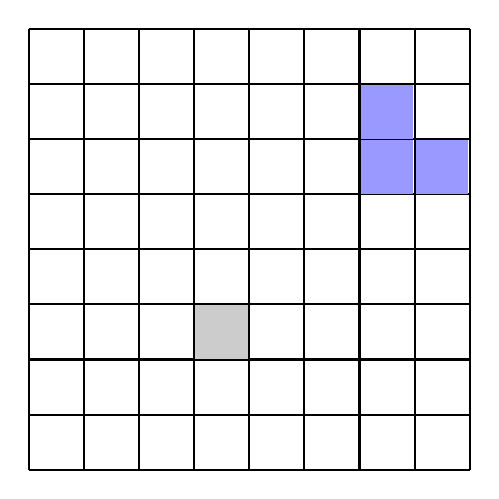
\begin{tikzpicture}[
	thick
]	
	\draw[step=0.7,black] (0.0,0.0) grid (5.6,5.6);
	\node[rectangle,anchor=north west,minimum width=0.67cm,minimum height=0.68cm,fill=gray!40] at (2.1,2.1) {};
	\node[rectangle,anchor=north west,minimum width=0.67cm,minimum height=0.68cm,fill=blue!40] at (4.2,4.2) {};
	\node[rectangle,anchor=north west,minimum width=0.67cm,minimum height=0.68cm,fill=blue!40] at (4.9,4.2) {};
	\node[rectangle,anchor=north west,minimum width=0.67cm,minimum height=0.68cm,fill=blue!40] at (4.2,4.9) {};
\end{tikzpicture}
}
\end{frame}

\section{Backtracking iterativo}

\subsection{Inviluppo convesso}

%-------------------------------------------------------------------------
\begin{frame}{Inviluppo convesso (Convex Hull)}

\vspace{-12pt}
\TwoCols{
\begin{myboxtitle}[Poligono convesso]
Un poligono nel piano è \alert{convesso} se ogni segmento di retta che
congiunge due punti del poligono sta interamente nel poligono stesso (bordo incluso).
\end{myboxtitle}
}{
\begin{myboxtitle}[Inviluppo convesso]
Dati $n$ punti $p_1, \ldots, p_n$ nel piano, con $n \geq 3$, l'\alert{inviluppo convesso}
(\alert{convex hull}) è, fra tutti i poligoni convessi che li contengono tutti, quello di superficie minima.
\end{myboxtitle}
}

\medskip
\IG{1.0}{16-back-geometry1.pdf}

\end{frame}

%-------------------------------------------------------------------------
\begin{frame}{"Stessa parte"}

\vspace{-9pt}
\begin{myboxtitle}[Problema]
Data una retta definita dai punti $p_1$ e $p_2$, determinare se due punti $p$ e $q$ 
stanno nello stesso semipiano definito dalla retta.
\end{myboxtitle}

\medskip
\begin{Procedure}
\caption[A]{\BOOLEAN\ \textsf{sameSide}(\Point $p_1$, \Point $p_2$, \Point $p$, \Point $q$)}
\REAL\ $dx = p_2.x - p_1.x$\;
\REAL\ $dy = p_2.y - p_1.y$\;
\REAL\ $dx_1 = p.x - p_1.x$\;
\REAL\ $dy_1 = p.y - p_1.y$\;
\REAL\ $dx_2 = q.x - p_2.x$\;
\REAL\ $dy_2 = q.y - p_2.y$\;
\Return $((dx \cdot dy_1 - dy \cdot dx_1) \cdot (dx \cdot dy_2 - dy \cdot dx_2) \ge 0)$\;
\end{Procedure}

\end{frame}


%-------------------------------------------------------------------------
\begin{frame}{Algoritmo inefficiente -- $O(n^3)$}

\BIL
\item Un poligono può essere rappresentato per mezzo dei suoi spigoli
\item Si consideri la retta che passa per una coppia di punti $p_i,p_j$, che divide il piano in due semipiani chiusi
\item Se tutti i rimanenti $n-2$ punti stanno "dalla stessa parte", allora lo
spigolo $S_{ij}$ fa parte dell’inviluppo convesso
\EIL
\IG{0.8}{16-back-geometry2.pdf}

\end{frame}


%-------------------------------------------------------------------------
\begin{frame}{Algoritmo di Jarvis (Gift Packing) -- $O(nh)$}

\BIL
\item Si considera il punto $p_0$ più basso, che appartiene sicuramente all'inviluppo convesso
\item Si seleziona il punto $p_{i+1}$ in modo tale che tutti gli altri punti siano a destra della retta passante per $p_i, p_{i+1}$
\item Questo punto può essere trovato in tempo $O(n)$ confrontando gli angoli formati dalla retta passante per $p_i, p_{i+1}$ e la retta passante per
$p_{i+1}, p_x$, per ogni punto $p_x$.
\item Il processo continua finchè il punto $p_x$ individuato è uguale a $p_0$
\EIL
\IG{0.8}{jarvis.pdf}

\end{frame}





%-------------------------------------------------------------------------
\begin{frame}{Algoritmo di Graham}

\vspace{-9pt}
\begin{myboxtitle}[Fase 1]
\BIL
\item Il punto con ordinata minima fa parte dell’inviluppo convesso
\item Si ordinano i punti in base all’angolo formato dalla retta passante per il punto con ordinata minima e la retta orizzontale
\EIL
\end{myboxtitle}

\IG{0.55}{16-back-geometry3.pdf}

\end{frame}

%-------------------------------------------------------------------------
\begin{frame}{Algoritmo di Graham}

\begin{Procedure}
\caption[A]{\Stack \graham($\Point[\,]\ p$, \INTEGER $n$)}
\INTEGER $\Min = 1$\;
\For{$i = 2$ \TO\ $n$}{
  \If{$p[i].y < p[\Min].y$}{$\Min = i$}
}
$p[1] \leftrightarrow p[\Min]$\;
\{ riordina $p[2, \mldots n]$ in base all'angolo formato rispetto all'asse orizzontale quando sono connessi con $p[1]$ \}\;
\{ elimina eventuali punti “allineati” tranne i più lontani da $p_1$, aggiornando $n$ \}\;
[...]\;
\end{Procedure}


\end{frame}

%-------------------------------------------------------------------------
\begin{frame}{Algoritmo di Graham}

\vspace{-9pt}
\begin{myboxtitle}[Fase 2]
\BIL
\item Inserisci $p_1,p_2$ nell'inviluppo corrente
\item Per tutti i punti $p_i = 3, \ldots, n$:
\BIL
\item Siano $p_{j-1}$ e $p_j$ il penultimo e ultimo vertice dell'inviluppo corrente
\item Se $\textsf{sameSide}(p_{j-1}, p_{j}, p_1, p_i) = \FALSE$, ovvero $p_1$ e $p_i$ non si trovano dalla stessa parte rispetto alla retta passante per $p_{j-1}$ e $p_j$, allora elimina $p_j$ dall'inviluppo corrente 
\item Termina tale "scansione" se $p_j$ non deve essere eliminato
\item aggiungi $p_i$ all'inviluppo “corrente”
\EIL
\EIL
\end{myboxtitle}

\end{frame}

%-------------------------------------------------------------------------
\begin{frame}{Algoritmo di Graham}

\vspace{-12pt}
\IG{0.65}{16-back-geometry4.pdf}

\end{frame}

%-------------------------------------------------------------------------
\begin{frame}{Algoritmo di Graham}

\begin{Procedure}
\caption[A]{\Stack \graham($\Point[\,]\ p$, \INTEGER $n$) (continua)}
$\Stack\ S = \stackconstructor()$\;
$S.\stackpush(p_1); S.\stackpush(p_2)$\;
\For{$i = 3$ \TO\ $n$}{
  \While{\NOT\ $\textsf{sameSide}(S.\stacktop(), S.\stacktopdue(), p_1, p_i)$}{
    $S.\stackpop()$\;
  }
  $S.\stackpush(p_i)$\;
}
\Return $S$\;  
\end{Procedure}


\end{frame}

%-------------------------------------------------------------------------
\begin{frame}{Conclusioni}

\vspace{-9pt}
\begin{myboxtitle}[Complessità dell'Algoritmo di Graham]
$O(n \log n)$, dominato dall'ordinamento
\end{myboxtitle}

\medskip
\begin{tabular}{|P{3cm}|P{5.8cm}|P{1.8cm}|}
\hline
\textbf{Algoritmo} & \textbf{Note} & \textbf{Compl.} \\\hline
Gift packing & $h$ numero di punti nell'inviluppo convesso (1973)& $O(nh)$\\\hline
Graham  & Backtracking iterativo (1972)& $O(n \log n)$\\\hline
Monotone Chain  & Come Graham, ma senza angoli (1979) & $O(n \log n)$ \\\hline
Preparata, Hong  & Divide et impera (1977) & $O(n \log n)$ \\\hline
Chan  & Graham + Jarvis (1996) & $O(n \log h)$ \\\hline
\end{tabular}




\end{frame}

%-------------------------------------------------------------------------
\begin{frame}{Conclusioni}


\BB{
“Convex hull is the favorite paradigm
of computational geometers.
Although the description of the problem is
fairly simple, its solution takes into account
all aspects of computational geometry.”
}


O. Devillers (1996)

\end{frame}


\begin{frame}{Quale tecnica applicare?}

\vspace{-9pt}
\begin{myboxtitle}[Sottostruttura ottima]
E' possibile spezzare ricorsivamente un problema in sottoproblemi più piccoli? Le decisioni prese per un problema rimangono valide quando esso diviene un sottoproblema di un problema più grande?
\end{myboxtitle}


\vspace{-9pt}
\begin{columns}[T]
\column{0.45\textwidth}
\BB{Risposta: S\`I}
\BIL
\item Divide-et-impera
\item Prog. dinamica
\item Memoization
\item Greedy
\item Backtrack
\EIL
\column{0.45\textwidth}
\BB{Risposta: NO}
\BIL
\item Backtrack
\item Oppure, risoluzione ad-hoc
\EIL
\end{columns}

\end{frame}

\begin{frame}{Quale tecnica applicare?}

\vspace{-9pt}
\begin{myboxtitle}[Spazio dei sottoproblemi]
Lo spazio dei sottoproblemi ha dimensione superpolinomiale?
\end{myboxtitle}

\vspace{-9pt}
\begin{columns}[T]

\column{0.45\textwidth}
\BB{Risposta: S\`I}
\BIL
\item Backtrack
\EIL

\column{0.45\textwidth}
\BB{Risposta: NO}
\BIL
\item Divide-et-impera
\item Prog. dinamica
\item Memoization
\item Greedy
\EIL

\end{columns}

\end{frame}


\begin{frame}{Quale tecnica applicare?}

\vspace{-9pt}
\begin{myboxtitle}[Ripetizioni]
Lo stesso sottoproblema può occorrere più volte come sottoproblema di un problema più grande?
\end{myboxtitle}

\vspace{-9pt}
\begin{columns}[T]
\column{0.45\textwidth}
\BB{Risposta: S\`I}
\BIL
\item Prog. dinamica
\item Memoization
\item Greedy
\EIL
\column{0.45\textwidth}
\BB{Risposta: NO}
\BIL
\item Divide-et-impera
\item Greedy
\EIL
\end{columns}

\end{frame}

\begin{frame}{Quale tecnica applicare?}

\vspace{-9pt}
\begin{myboxtitle}[Copertura dei sottoproblemi]
\BIL
\item Per risolvere il problema principale, è necessario risolvere tutti i sottoproblemi?
\EIL
\end{myboxtitle}

\vspace{-9pt}
\begin{columns}[T]
\column{0.45\textwidth}
\BB{Risposta: S\`I}
\BIL
\item Prog. dinamica
\item Memoization
\EIL
\column{0.45\textwidth}
\BB{Risposta: NO}
\BIL
\item Greedy
\item Memoization
\EIL
\end{columns}

\end{frame}


\end{document}



